\documentclass{book}[oneside]
\usepackage{CJKutf8}
\usepackage{amsmath}
\usepackage{amsfonts}
\usepackage{amsthm}
\usepackage{titlesec}
\usepackage{titletoc}
\usepackage{xCJKnumb}
\usepackage{graphicx}


\usepackage{tikz}
\titleformat{\chapter}{\centering\Huge\bfseries}{第\, \xCJKnumber{\thechapter}\,
    章}{1em}{}
  % \renewcommand{\chaptermark}[1]{\markboth{第 \thechapter 章}{}}
\usepackage{mathrsfs}

\newtheorem{Def}{定义}[chapter]
\newtheorem{Thm}{定理}[chapter]
\newtheorem{Cor}{推论}[chapter]
\newtheorem{Ax}{公理}[chapter]

\newtheorem{Exercise}{练习}[chapter]


\newtheorem{Example}{例}[chapter]


\begin{document}
\begin{CJK*}{UTF8}{gbsn}
  \title{离散数学讲义}
  \author{陈建文}
  \maketitle
  % \tableofcontents
  

  \setcounter{chapter}{8}
  \chapter{平面图和图的着色}
  \begin{Def}
    图$G$称为被嵌入平(曲)面$S$内,如果$G$的图解已画在$S$上,而且任意两条边均不相交(除可能在端点相交外)。
已嵌入平面内的图称为{\bfseries 平面图}。如果一个图可以嵌入平面,则称此图为{\bfseries 可平面的}。
\end{Def}
  \begin{Def}
    平面图$G$把平面分成了若干个区域,这些区域都是连通的,称之为$G$的面,其中无界的那个连通区域称为$G$的外部面,其余的连通区域称为$G$的内部面。
  \end{Def}
  \begin{center}
  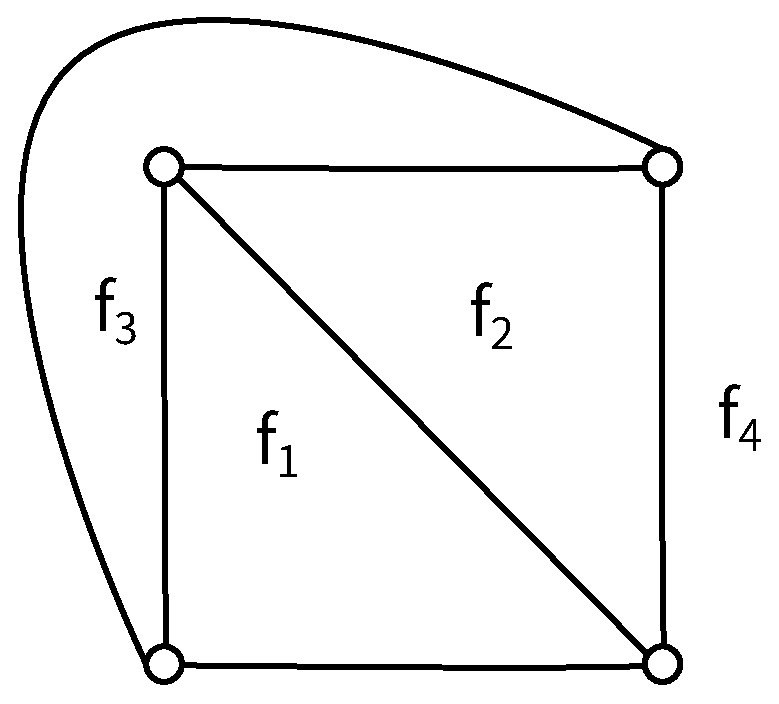
\includegraphics[width=4cm,height=3cm]{face}
\end{center}
\begin{Thm}[欧拉公式]
    如果有$p$个顶点$q$条边的平面连通图$G$有$f$个面,则
      $p - q + f = 2$
    \end{Thm}
    \begin{proof}[证明]
\mbox{}\par{}
    用数学归纳法证明,施归纳于面数$f$。

  (1)当$f=1$时,$G$中无圈,又因为$G$是连通的,所以$G$是树。从而
  $q=p-1$,$p-q+f=2$成立。

  (2)假设当$f=k$时结论成立,往证当$f=k+1$时结论也成立。假设$G$有$k+1$个面,
  $k\geq 1$。此时$G$至少有一个内部面,从而有一个圈。从这个圈上去掉一条边$x$,则
  $G-x$就是一个有$p$个顶点,$q-1$条边,$k$个面的平面连通图。由归纳假设,对
  $G-x$结论成立,即\[p-(q-1) + k =2\]
  因此,\[p-q+ (k+1) =2\]
  即当$f=k+1$时结论也成立。
\end{proof}
 \begin{Cor}
    若平面图$G$有$p$个顶点$q$条边且每个面都是由长为$n$的圈围成的,则
    \begin{equation*}
      q = n(p-2)/(n-2)
    \end{equation*}
  \end{Cor}
一个{\bfseries 最大可平面图}是一个可平面图,对此可平面图中不能再加入边而不破坏其可平面性。
  \begin{Cor}
    设$G$为一个有$p$个顶点$q$条边的最大可平面图,$p \geq 3$,则$G$的每个面都为三角形,而且$q=3p-6$。
  \end{Cor}
  \begin{Cor}
    设$G$为一个$(p,q)$可平面连通图,而且$G$的每个面都是由一个长为$4$的圈围成的,则$q=2p-4$。
  \end{Cor}
  \begin{Cor}
    若$G$为一个有$p$个顶点$q$条边的可平面图,$p\geq 3$,则$q \leq 3p - 6$;进一步,若$G$中没有三角形,则$q \leq 2p -4$。
  \end{Cor}
     \centering
    \begin{tikzpicture}[auto,
    specification/.style ={circle, draw, thick, inner sep = 0pt, minimum size=2mm}]
   \node[specification] (A)  at (0:2cm)  {};
   \node[specification] (B)  at (60:2cm)  {};
   \node[specification] (C)  at (120:2cm)  {};
   \node[specification] (D) at (180:2cm)  {};
   \node[specification] (E)  at (240:2cm)  {};   
   \node[specification] (F)  at (300:2cm)  {};   
   \node[specification] (G)  at (300:0.5cm)  {};
   \node[specification] (H)  at (180:3cm)  {};
   
   
   \draw[thick] (A) to  (B);
   \draw[thick] (B) to  (C);
   \draw[thick] (C) to  (D);
   \draw[thick] (D) to  (E);
   \draw[thick] (E) to  (F);
   \draw[thick] (F) to  (A);
   \draw[thick] (B) to  (E);
   \draw[thick] (F) to  (G);
   \draw[thick] (D) to  (H);   
 \end{tikzpicture}
 \begin{proof}[证明]
  不妨设$G$为连通的可平面图,否则可以加边使之变成连通的。由于每个面至少含有3条边,因此
  \[2q \geq 3f\]
  即
  \[\frac{2q}{3} \geq f\]
  因此,根据欧拉公式
  \[p - q + f = 2\]
  得
  \[p - q + \frac{2q}{3} \geq 2\]
  化简得:
  \[q \leq 3p - 6\]

  进一步,若$G$中没有三角形,则$G$中的每个面至少含有4条边,因此
  \[2q \geq 4f\]
  即
  \[\frac{q}{2} \geq f\]
  因此,根据欧拉公式
  \[p-q+f=2\]
  得
  \[p-q+ \frac{q}{2} \geq 2\]
  化简得:
  \[q \leq 2p - 4\]
\end{proof}

  \begin{Cor}
    $K_5$和$K_{3,3}$都不是可平面图。
  \end{Cor}
\vspace{1cm}
  \begin{minipage}{0.45\linewidth}
      \centering
    \begin{tikzpicture}[auto,
    specification/.style ={circle, draw, thick}]
   \node[specification] (A)   at (18:1.3cm)  {};
   \node[specification] (B)   at (90:1.3cm)  {};
   \node[specification] (C)   at (162:1.3cm)  {};
   \node[specification] (D)  at (234:1.3cm)  {};
   \node[specification] (E)   at (306:1.3cm)  {};      
   
   
   \draw[thick] (A) to  (B);
   \draw[thick] (B) to  (C);
   \draw[thick] (C) to  (D);
   \draw[thick] (D) to  (E);
   \draw[thick] (E) to  (A);
   \draw[thick] (A) to  (C);
   \draw[thick] (B) to  (E);
   \draw[thick] (C) to  (E);
   \draw[thick] (D) to  (A);
   \draw[thick] (B) to  (D);
 \end{tikzpicture}
    
  \end{minipage}
  \begin{minipage}{0.45\linewidth}
    \centering
    \begin{tikzpicture}[auto,
    specification/.style ={circle, draw, thick}]
   \node[specification] (A) at (0,0)  {};
   \node[specification] (B) at (1,0)  {};
   \node[specification] (C) at (2,0)  {};
   \node[specification] (D) at (0,1)  {};
   \node[specification] (E) at (1,1)  {};
   \node[specification] (F) at (2,1)  {};
   \draw[thick] (A) to  (D);
   \draw[thick] (A) to  (E);
   \draw[thick] (A) to (F);
   \draw[thick] (B) to (D);
   \draw[thick] (B) to (E);
   \draw[thick] (B) to (F);
   \draw[thick] (C) to (D);
   \draw[thick] (C) to (E);
   \draw[thick] (C) to (F);
 \end{tikzpicture}
  \end{minipage}
  \begin{proof}[证明]
  先证明$K_5$不是可平面图。用反证法,假设$K_5$为可平面图,其顶点数$p = 5$, 边数$q = 10$,此时
  \[q \leq 3p - 6\]
  即
  \[10 \leq 3 \times 5 - 6 = 9\]
  矛盾。因此$K_5$不是可平面图。

  接下来证明$K_{3,3}$不是可平面图。用反证法,假设$K_{3,3}$为可平面图,其顶点数为$p=6$,边数$q=9$,由$K_{3,3}$中没有三角形知
  \[q \leq 2p -4\]
  即
  \[9 \leq 2 * 6 - 4 = 8\]
  矛盾。因此$K_{3,3}$不是可平面图。
\end{proof}
  \begin{Cor}
    每个可平面图$G$中顶点度的最小值不超过5,即$\delta (G) \leq 5$。
  \end{Cor}
  \begin{proof}[证明(证法一)]
  当图$G$的顶点数$p=1,2$时,结论显然成立。当$p\geq 3$时,
  设可平面图$G$有$q$条边,则
  \[\delta p \leq 2q\]
  由$G$为可平面图知
  \[q \leq 3p - 6\]
  从而
  \[\delta p \leq 6p - 12\]
  两边同时除以$p$,得:
  \[\delta \leq 6 - \frac{12}{p}\]
  即
  \[\delta \leq 5\]
\end{proof}
\begin{proof}[证明(证法二)]
  当图$G$的顶点数$p=1,2$时,结论显然成立。
  当$p \geq 3$时,用反证法证明结论也成立。假设$\delta (G) \geq 6$,设$G$有$q$条边,则
  \[6p \leq 2q\]
  由$G$为可平面图知
  \[q \leq 3p - 6\]
  从而
  \[6p \leq 6p - 12\]
矛盾。  
\end{proof}

  \begin{Thm}
    设$G=(V,E)$为一个$(p,q)$平面哈密顿图,$C$为$G$的哈密顿圈。
    令$f_i$为$C$的内部由$i$条边围成的面的个数,$g_i$为$C$的外部$i$条边围成的面的个数,则
    \begin{align}
      &1 \cdot f_3 + 2 \cdot f_4 + 3 \cdot f_5 + \cdots = \sum_{i=3}^p(i-2)f_i = p - 2;\\
      &1 \cdot g_3 + 2 \cdot g_4 + 3 \cdot g_5 + \cdots = \sum_{i=3}^p(i-2)g_i = p - 2;\\
      &1 \cdot (f_3 - g_3) + 2 \cdot (f_4 - g_4) + 3 \cdot (f_5 - g_5) + \cdots = \sum_{i=3}^p(i-2)(f_i - g_i) = 0
    \end{align}
  \end{Thm}
    \centering
  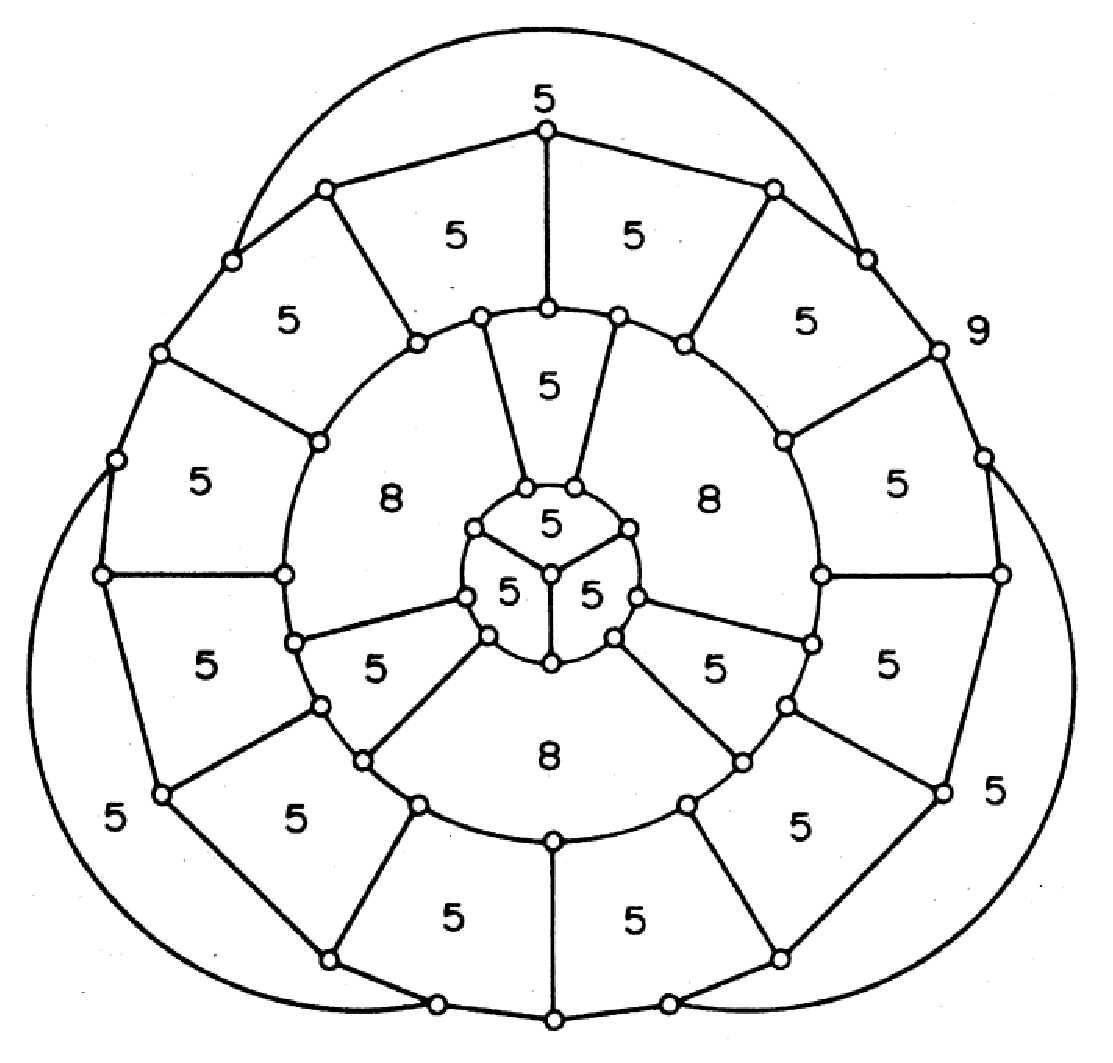
\includegraphics[width=7cm, height=6cm]{grinberg}
  \begin{Def}
    设$x=uv$为图$G=(V,E)$的一条边,又$w$不是$G$的顶点,则当用边$uw$和$wv$代替边$x$时,就称$x$被细分。如果$G$的某些条边被细分,产生的图称为$G$的细分图。
  \end{Def}
  \begin{Def}
    两个图称为同胚的,如果它们都可以从同一个图通过一系列的边细分得到。
  \end{Def}
  \begin{Thm}
    一个图为可平面的充分必要条件是它没有同胚于$K_5$或$K_{3,3}$的子图。
  \end{Thm}
  \begin{Def}
    一个图$G$的一个初等收缩由等同两个临接的顶点$u$和$v$得到,即从$G$中去掉$u$和$v$,然后再加上一个新顶点$w$,使得$w$临接于所有临接于$u$或$v$的顶点。一个图$G$可以收缩到图$H$,如果$H$可以从$G$经过一系列的初等收缩得到。
  \end{Def}
  \begin{Thm}
    一个图为可平面的当且仅当它没有一个可以收缩到$K_5$或$K_{3,3}$的子图。
  \end{Thm}
  \begin{Def}
    设$G=(V,E)$为一个平面图,由$G$按照如下方法构造一个图$G^*$,$G^*$称为$G$的对偶图:对$G$的每个面$f$对应地有$G^*$的一个顶点$f^*$;对$G$的每条边$e$对应地有$G^*$的一条边$e^*$:$G^*$的两个顶点$f^*$与$g^*$由边$e^*$联结,当且仅当$G$中与顶点$f^*$与$g^*$对应的面$f$与$g$有公共边$e$,如果某条边$x$仅在一个面中出现而不是两个面的公共边,则在$G^*$中这个面对应的顶点有一个环。
  \end{Def}
  \begin{Def}
    图的一种{\bfseries 着色}是指对图的每个顶点指定一种颜色,使得没有两个临接的顶点有同一种颜色。图$G$的一个{\bfseries $n-$着色}是用$n$种颜色对$G$的着色。
  \end{Def}
  \begin{Def}
    图$G$的{\bfseries 色数}是使$G$为$n-$着色的数$n$的最小值,图$G$的色数记为$\chi(G)$。若$\chi (G) \leq n$,则称$G$为{\bfseries $n-$可着色}的。若$\chi (G) = n$,则称$G$为{\bfseries $n$色}的。
  \end{Def}
  \begin{Thm}
    一个图是可双色的当且仅当它没有奇数长的圈。
  \end{Thm}
  \renewcommand{\figurename}{图}
\begin{figure}\centering
  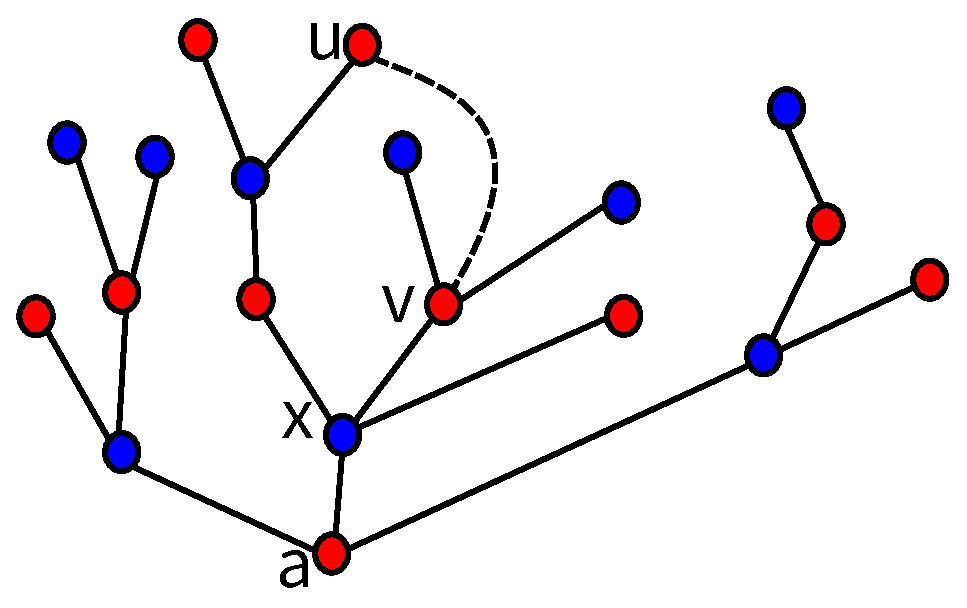
\includegraphics[width=4cm,height=3cm]{color26}
      \caption{用两种颜色对一个没有奇数长的圈的图进行着色的示意图}
    \label{fig:twocoloring}  
    \end{figure}
    \begin{proof}[证明]
    设图$G$为可双色的,则显然图$G$没有奇数长的圈。这是因为假设图$G$有奇数长的圈$C$,
    则$C$是3色的,从而$\chi(G) \geq 3$,与$G$是可双色的矛盾。

      设图$G$没有奇数长的圈,以下给出一种用两种颜色对$G$的顶点进行着色的算法,从而证明图$G$是可双色的。不妨设图$G$是连通的,否则可以对图$G$的每个连通分量分别进行着色。任取$G$的一个顶点$a$,对其着红色,然后对与顶点$a$邻接的顶点着蓝色,接下来对所有与已经着色的顶点相邻接的顶点着红色,这样依次下去,每次都对所有与已经着色的顶点相邻接的顶点着与前一次的着色不同的另一种颜色。如图~\ref{fig:twocoloring}所示该算法结束时用至多两种颜色对$G$的顶点进行了着色。

以下证明每次对所有与已经着色的顶点相邻接的顶点着与前一次的着色不同的另一种颜色时,
不会产生相邻的两个顶点着以相同颜色的情况,从而保证前面的算法是正确的。用反证法。
假设对顶点$u$进行着色时,不妨设对其着红色,已经有一个与之相邻的顶点$v$着了红色。
从着色的过程知,从顶点$a$到顶点$u$之间有一条路$P_1$,其上的顶点依次着了红色和蓝色,
从顶点$a$到顶点$v$之间也有一条路$P_2$,其上的顶点依次着了红色和蓝色。
取$P_1$和$P_2$的最后一个公共的顶点$x$,则$P_1$上从顶点$u$到顶点$x$的路与$P_2$上从顶点$x$到顶点$v$的路和边$vu$一起构成一个圈,该圈上$u$和$v$着相同的颜色,其他各顶点依次着不同的颜色,因此其长度为奇数,与$G$中没有奇数长的圈矛盾。 
  \end{proof}

  \begin{Thm}
    设$\Delta = \Delta (G)$为图$G$的顶点度的最大值,则$G$为$(\Delta+1)-$可着色的。
  \end{Thm}
  \begin{proof}[证明]用数学归纳法证明,施归纳于顶点数$p$。

    (1)当$p=1$时,结论显然成立。

    (2)假设当$p=k(k\geq 1)$时结论成立,往证当$p=k+1$时结论也成立。设$v$为$G$中的任意一个顶点,由归纳假设,$G-v$是$\Delta(G-v)+1$可着色的。又由于$\Delta(G-v) \leq \Delta$,从而$G-v$为$\Delta+1$可着色的。假设已经用至多$\Delta+1$种颜色对$G-v$进行了顶点着色,使得任意相邻的顶点着不同的颜色,那么此时在$G$中与$v$邻接的顶点用了至多$\Delta$种颜色,用另外一种不同的颜色对顶点$v$进行着色,从而用至多$\Delta+1$种颜色就可以对$G$的顶点进行着色使得相邻的顶点着不同的颜色,即$G$为$\Delta + 1$可着色的。
    
  \end{proof}
  \clearpage
  \begin{Thm}
    如果$G$是一个连通图且不是完全图也不是奇数长的圈,则$G$为$\Delta(G)-$可着色的。
  \end{Thm}

  \begin{proof}[证明]
    用数学归纳法证明,施归纳于顶点数$p$。

   (1)当$p=1$时,结论显然成立。

   (2)假设当$p<k(k\geq 2)$时结论成立,往证当$p=k$时结论也成立。设图$G$为有$k$个顶点的连通图,$G$不是完全图也不是奇数长的圈,$v$为图$G$的任意一个顶点。考虑$G-v$的每个支$H$。如果$H$不是完全图也不是奇数长的圈,由归纳假设,$\chi(H)\leq \Delta(H) \leq \Delta(G)$;如果$H$为完全图或者奇数长的圈,因为$H$中有一个顶点与$v$之间有边相连,所以$\chi(H) = \Delta(H) + 1 \leq \Delta(G)$。总之,$G-v$的每个支$H$为$\Delta(G)$可着色的,因此$G-v$为$\Delta(G)$可着色的。

   如果$\deg v \leq \Delta(G)-1$,则在$G-v$中用至多$\Delta(G)$种颜色进行顶点着色时,在$G$中与$v$邻接的顶点至多用了$\Delta(G)-1$种颜色,此时,用另外一种不同的颜色对顶点$v$进行着色,这样用至多$\Delta(G)$种颜色就可以对$G$的顶点进行着色,从而图$G$为$\Delta(G)-$可着色的。

   以下考虑$\deg v = \Delta(G)$的情况。此时与$v$邻接的$\Delta(G)$个顶点$v_1,v_2,\ldots,v_{\Delta(G)}$在$G-v$中分别用颜色$c_1,c_2,\ldots,c_{\Delta(G)}$进行了着色。如果$c_1,c_2,\ldots,c_{\Delta(G)}$中有两种颜色是相同的,则$c_1$, $c_2$, $\ldots$, $c_{\Delta(G)}$中至多有$\Delta(G)-1$种颜色,用另外一种颜色对顶点$v$进行着色,这样用至多$\Delta(G)$种颜色就可以对$G$的顶点进行着色。以下考虑$c_1,c_2,\ldots,c_{\Delta(G)}$中的各种颜色互不相同的情况。对任意的正整数$i$,$j$,$i\neq j$,设$H_{ij}$为着颜色$c_i$和$c_j$的顶点集的导出子图。此时,分以下情况讨论:

   (1)如果存在正整数$i$,$j$,$i\neq j$,顶点$v_i$和顶点$v_j$位于$H_{ij}$的不同的支中,交换$v_i$所在的支中顶点的着色,即着颜色$c_i$的顶点改着颜色$c_j$,着颜色$c_j$的顶点改着颜色$c_i$,于是顶点$v_i$和顶点$v_j$都用颜色$c_j$进行了着色,用颜色$c_i$对顶点$v$进行着色,这样用$\Delta(G)$种颜色就可以对$G$的顶点进行着色。

   (2)如果对任意的正整数$i$,$j$,$i\neq j$,顶点$v_i$和顶点$v_j$都位于$H_{ij}$的同一个支$C_{ij}$中。设$P_{ij}$为$C_{ij}$中从$v_i$到$v_j$的一条路。在$C_{ij}$中,如果$\deg v_i>1$,则在$G-v$中与顶点$v_i$邻接的至多$\Delta(G)-1$个顶点中至多用了$\Delta(G)-2$种颜色,用除颜色$c_i$之外的另外一种多余的颜色对顶点$v_i$进行着色,然后用颜色$c_i$对顶点$v$进行着色,这样用$\Delta(G)$种颜色就可以对$G$的顶点进行着色。类似的,在$C_{ij}$中,如果$\deg v_j>1$,也可以用$\Delta(G)$种颜色对$G$的顶点进行着色。如果以上两种情况都不成立,设$u\neq v_i,v_j$为$P_{ij}$中某个顶点,在$C_{ij}$中,$\deg u>2$,则在$G-v$中与顶点$u$邻接的顶点至多用了$\Delta(G)-2$种颜色,用除顶点$u$所着颜色之外的另一种颜色对顶点$u$进行着色,可以划归为情况(1)。因此以下考虑对任意的$C_{ij}$,$C_{ij}$为从顶点$v_i$到顶点$v_j$的一条路的情况。此时如果$\deg v=2$,则$\Delta(G)=2$,$G$为奇数长的圈,矛盾。以下考虑$\deg v\geq 3$的情况。如果存在不同的正整数$i,j,k$,$C_{ij}$与$C_{ik}$有一个除了$v_i$之外的公共顶点$u$,此时顶点$u$有两个与之邻接的顶点着了颜色$c_j$,另外还有两个与之邻接的顶点着了颜色$c_k$,于是与顶点$u$邻接的顶点至多用了$\Delta(G)-2$种颜色,用除了顶点$u$所着颜色之外的另一种颜色对顶点$u$进行着色,可以划归为情况(1)。以下考虑对任意不同的正整数$i,j,k$,$C_{ij}$与$C_{ik}$除了顶点$v_i$之外没有其他的公共顶点的情况。此时与$v$邻接的顶点$v_1,v_2,\ldots,v_{\Delta(G)}$中必有两个是不邻接的,这是因为如果$v_1,v_2,\ldots,v_{\Delta(G)}$两两邻接,它们又都与$v$邻接,这就构成了一个包含$\Delta(G)+1$个顶点的完全图,与$G$不是完全图矛盾。不妨设$v_1$和$v_2$为与$v$邻接的顶点中不邻接的两个顶点。设$u$为$C_{12}$中与$v_1$邻接的顶点,则在$G-v$中$u$着了颜色$c_2$。交换$C_{13}$中各顶点的颜色,即着颜色$c_1$的顶点改着颜色$c_3$,着颜色$c_3$的顶点改着颜色$c_1$。重新考虑$G-v$中各顶点的着色,此时如果$v_1$和$v_2$位于$H_{12}$的不同的支中,或$v_2$和$v_3$位于$H_{23}$的不同的支中,则划归为情况(1)。否则,如果$C_{12}$不是路,或者$C_{23}$不是路,则按照前面叙述的方法可以用$\Delta(G)$种颜色对$G$的顶点进行着色。最后,如果$C_{12}$和$C_{23}$都为路,此时$u$为$C_{12}$和$C_{23}$的除了$v_2$之外的公共顶点,亦可以采用前面叙述的方法用$\Delta(G)$种颜色对$G$的顶点进行着色。

   
   
  \end{proof}
  \begin{Thm}
    每个平面图为$6-$可着色的。
  \end{Thm}
   \begin{proof}[证明]
   用数学归纳法证明,施归纳于顶点数$p$。

   (1)当$p=1$时,结论显然成立。

   (2)假设当$p=k(k\geq 1)$时结论成立,往证当$p=k+1$时结论也成立。设平面图$G$有$k+1$个顶点,则图$G$中一定有一个顶点$v$使得$\deg v \leq 5$。于是,$G-v$是一个有$k$个顶点的平面图,由归纳假设,$G-v$是$6-$可着色的。假设用至多$6$种颜色对$G-v$进行了着色。由于$\deg v \leq 5$,在$G-v$中用至多$6$种颜色进行顶点着色时,在$G$中与$v$邻接的顶点至多用了$5$种颜色。此时,用另外一种不同的颜色对顶点$v$进行着色,这样用至多$6$种颜色就可以对$G$的顶点进行着色,从而图$G$为$6-$可着色的。
  \end{proof}

  \begin{Thm}
    每个平面图为$5-$可着色的。
  \end{Thm}
  \begin{proof}[证明]
  用数学归纳法证明,施归纳于图的顶点数$p$。

  (1)当$p=1$时,结论显然成立。

  (2)假设当$p<k$时结论成立,往证当$p=k$时结论也成立。设平面图$G$有$k$个顶点,则图$G$中一定有一个顶点$v$使得$\deg v \leq 5$。于是,$G-v$是一个有$k-1$个顶点的平面图,由归纳假设,$G-v$是$5-$可着色的。假设用至多5种颜色对$G-v$进行了着色。

  如果$\deg v \leq 4$,则在$G-v$中用至多5种颜色进行顶点着色时,在$G$中与$v$邻接的顶点至多用了$4$种颜色,如图~\ref{fig:coloring}所示。此时,用另外一种不同的颜色对顶点$v$进行着色,这样用至多5种颜色就可以对$G$的顶点进行着色,从而图$G$是$5-$可着色的。
\begin{figure}
  \begin{minipage}{0.49\linewidth}
    \centering
   \begin{tikzpicture}[auto,
    specification/.style ={circle, draw, thick, inner sep = 0pt, minimum size=2mm}]
   \node[specification, fill = blue] (A)  [label=0:$v_1$] at (18:1.3cm)  {};
   \node[specification, fill = red] (C)  [label=180:$v_4$] at (162:1.3cm)  {};
   \node[specification, fill = green] (D) [label=180:$v_3$] at (234:1.3cm)  {};
   \node[specification, fill = orange] (E)  [label=0:$v_2$] at (306:1.3cm)  {};      
   \node[specification] (o)  [label=0:$v$] at (0,0)  {};      
   \draw[thick] (A) to  (o);
   \draw[thick] (C) to  (o);
   \draw[thick] (D) to  (o);
   \draw[thick] (E) to  (o);
 \end{tikzpicture}
    \caption{$\deg v \leq 4$的情况}
    \label{fig:coloring}  
  \end{minipage}
  \begin{minipage}{0.49\linewidth}
    \centering
   \begin{tikzpicture}[auto,
    specification/.style ={circle, draw, thick, inner sep = 0pt, minimum size=2mm}]
   \node[specification, fill = blue] (A)  [label=0:$v_2$] at (18:1.3cm)  {};
   \node[specification, fill = purple] (B)  [label=90:$v_1$] at (90:1.3cm)  {};
   \node[specification, fill = red] (C)  [label=180:$v_5$] at (162:1.3cm)  {};
   \node[specification, fill = green] (D) [label=180:$v_4$] at (234:1.3cm)  {};
   \node[specification, fill = orange] (E)  [label=0:$v_3$] at (306:1.3cm)  {};      
   \node[specification] (o)  [label=0:$v$] at (0,0)  {};      
   
   
   \draw[thick] (A) to  (o);
   \draw[thick] (B) to  (o);
   \draw[thick] (C) to  (o);
   \draw[thick] (D) to  (o);
   \draw[thick] (E) to  (o);
 \end{tikzpicture}
  \caption{$\deg v = 5$的情况}
  \label{fig:collision}
  \end{minipage}
\end{figure}    


如果$\deg v = 5$,与$v$邻接的$5$个顶点$v_1,v_2,v_3,v_4,v_5$在$G-v$中用$c_1,c_2,c_3,c_4,c_5$ 5种颜色进行了着色。如果$c_1,c_2,c_3,c_4,c_5$中有两种颜色是相同的,则$c_1$, $c_2$, $c_3$, $c_4$, $c_5$中至多有$4$种颜色,用另外一种颜色对顶点$v$进行着色,这样用至多5种颜色就可以对$G$的顶点进行着色。以下考虑$c_1,c_2,c_3,c_4,c_5$中的各种颜色互不相同的情况,如图~\ref{fig:collision}所示。在图$G$中,与顶点$v$邻接的$5$个顶点$v_1,v_2,v_3,v_4,v_5$中一定有两个顶点是不邻接的,否则图$G$中将有一个子图$K_5$,这与图$G$为平面图相矛盾。取其中不邻接的两个顶点$v_i$和$v_j$,在$G-v$中,将顶点$v_i$和顶点$v_j$视为同一个顶点$w$,即去掉顶点$v_i$和$v_j$,添加一个新的顶点$w$,原来与顶点$v_i$和顶点$v_j$相关联的边变为与顶点$w$相关联的边,得到的新的图记为$G'$,则$G'$仍然为平面图。由归纳假设,$G'$为$5-$可着色的。 设用至多$5$种颜色对$G'$进行了顶点着色。在$G-v$中,顶点$v_i$和顶点$v_j$都着与$w$相同的颜色,其他的顶点均与$G'$中相对应的顶点着相同的颜色,这样$G-v$用至多5种颜色就可以进行顶点着色。在这里,在$G$中与顶点$v$邻接的五个顶点$v_1,v_2,v_3,v_4,v_5$中用了4种颜色,用另外一种颜色对顶点$v$着色,这样用至多5种颜色就可以对$G$的顶点进行着色,从而图$G$为$5-$可着色的。
\end{proof}

  \begin{Thm}
    每个平面图为$4-$可着色的。
  \end{Thm}

\chapter{}

\end{CJK*}
\end{document}





%%% Local Variables:
%%% mode: latex
%%% TeX-master: t
%%% End:



